\documentclass{beamer}
\usetheme{Copenhagen}
\usepackage{polyglossia}
\usepackage{tabu}
\setdefaultlanguage{german}
\beamertemplatenavigationsymbolsempty

\title{Socio-Technical Distillation}
\subtitle{From Micro-Level Responsibilities to Macro-Level Architecture Views}

%\usetheme{lucid}
\begin{document}
	\frame {
		\titlepage
		\centering
		
\includegraphics[scale=0.25]{OTH_LOGO.png}
	}
	%\begin{frame}
	%\frametitle{Topics}
	%	\begin{block}{}

	%	\end{block}
	%\end{frame}

	%$\Rightarrow$

	\begin{frame}
	\frametitle{Themeneinführung}
		\begin{block}{Organisation großer Softwareprojekte}
			\begin{itemize}
				\item Große Softwaresysteme benötigen viel Kooperation
				%\item Verständnis und Dokumentation des Softwaresystems extrem wichtig
				\item Hunderte/Tausende Entwickler, die Arbeit koordinieren
			\end{itemize}
		\end{block}

		$\Rightarrow$ wohldefinierter Entwicklungsprozesses nötig, um Code-Review, Code-Integration, o.Ä. sicherzustellen
	\end{frame}

	\begin{frame}
	\frametitle{Themeneinführung}
		\begin{block}{Linux Kernel Entwicklungsprozess}
			\begin{itemize}
				\item Linux Kernel: weltweit verbreitetes Open Source Betriebssystem
				\item Offener Entwicklungsprozess auf Mailinglisten
				\item Zu großer Verwaltungsaufwand für einzelne Entwickler
			\end{itemize}
		\end{block}
		\centering
		$\Rightarrow$ Aufteilung des Codes in Verantwortungsbereiche, beaufsichtigt von Entwicklern, sog. \textit{Maintainers}

		$\Rightarrow$ Viele andere offen entwickelte Softwaresysteme lehnen sich an dieses Entwicklungsprozessmodell an (QEMU, U-Boot, Xen-Project)
	\end{frame}

	\begin{frame}
	\frametitle{Themeneinführung}
		\begin{block}{Maintainers}
			\begin{itemize}
				\item Erfahrene Entwickler für ihren Verantwortungsbereich
				\item Hauptaufgabe: neuen Code in ihrem Bereich integrieren, Gewährleistung für Codequalität
				\item Maintainers Experten in deren Bereichen, aber andere Teile des Projektes... ?
				\item Unkonforme Integrationen möglich
			\end{itemize}
		\end{block}

		\centering
		$\Rightarrow$ Verletzung des Entwicklungsprozesses

		$\Rightarrow$ mögliche Auswirkung auf Codequalität

		$\Rightarrow$ Effekt auf zahlreiche Systeme weltweit

		%\begin{alertblock}{Forschungsfrage: Integration von Patches?}
		%	Integration innerhalb der letzten Monate von zuständigen Maintainern?
		%\end{alertblock}

	\end{frame}

	\begin{frame}
	\frametitle{Themeneinführung}
		\begin{block}{Dokumentation}
			\begin{itemize}
				\item Software ändert sich ständig bei Weiterentwicklung
				\item Dokumentation enthält oft veraltete (manchmal falsche) Informationen
				\item Instandhaltung der Dokumentation wird nicht oft/hoch priorisiert
				\item Automatisierte Software-Architekturen aus Source Code trotz viel Forschung noch sehr unzufriedenstellend
			\end{itemize}
		\end{block}
	\end{frame}

	\begin{frame}
	\frametitle{Ziele}
		\begin{block}{Von Verantwortlichkeit zu Architektur}
			\begin{itemize}
				\item Manuelle menschliche Dokumentation oft vernachlässigt
				\item Allerdings: gut gepflegte Verantwortlichkeit-Informationen
				\item Code-Verantwortlichkeiten $\Rightarrow$ Rückschlüsse über Architektur
			\end{itemize}
		\end{block}
	\end{frame}

	\begin{frame}
	\frametitle{Forschungsbeiträge der Masterarbeit}
		\begin{alertblock}{Multi-Stepped Ansatz um Architektursysteme zu distillieren}
			\begin{enumerate}	
				\item Methodik: Existente Artefakte \textit{implizieren} Strukturen $\Rightarrow$ Architekturansicht generieren
				\item Usecase: Integrationsanalysen
				\item Methodik/Usecase statistisch verifizieren
			\end{enumerate}
		\end{alertblock}
	\end{frame}

	\begin{frame}
	\frametitle{Analysierte Projekte}
		\begin{block}{Analysierte Projekte}
			\begin{itemize}
				\item Linux
				\item QEMU
				\item U-Boot
				\item Xen-Project
			\end{itemize}
		\end{block}
	\end{frame}


	\begin{frame}
	\frametitle{Konzepte}
		\begin{center}
			\Huge Konzepte für offene Entwicklungsprozesse
		\end{center}
		%\begin{center}
		%	\begin{enumerate}
		%		\item get\_maintainer.pl Skript
		%		\item MAINTAINERS-Datei
		%	\end{enumerate}
		%\end{center}
		
	\end{frame}

	%\begin{frame}
	%\frametitle{Skripte}
	%	\begin{block}{Hilfestellung für Developer}
	%		\begin{itemize}
	%			\item Neuer Patch entwickelt $\Rightarrow$ auf relevante Mailinglists und zuständigen Maintainern schicken
	%			\item Problem: Woher bekommt man die notwendigen Informationen?
	%			%\item Relevante Maintainers und Listen in grdokumentiert, aber fehlende Übersichtsstruktur
	%		\end{itemize}
	%	\end{block}
	%	$\Rightarrow$ Jedes Projekt besitzt eigenes Skript zur Ausgabe von relevanten Listen und Personen
	%\end{frame}

	%\begin{frame}
	%\frametitle{Skripte}
	%	\begin{block}{Nutzung}
	%		Datei/Ordner/Patch als Input für Skript $\Rightarrow$ relevante Maintainers, Mailinglisten und Verantwortungsbereiche als Output
	%	\end{block}

	%	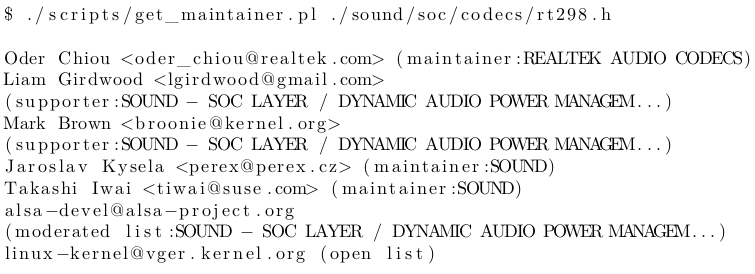
\includegraphics[scale=0.25]{Bilder/getmaintaineroutput.png}
	%\end{frame}

	\begin{frame}
	\frametitle{MAINTAINERS-Datei}
		\begin{block}{MAINTAINERS}
			MAINTAINERS ist eine Datei, die ...
			\begin{itemize}
				\item ... alle relevanten Maintainer und Personen...
				\item ... alle relevanten Mailinglisten...
				\item ... alle relevanten Zusatzinformationen...
			\end{itemize}
			... für alle Verantwortungsbereiche dokumentiert.

		\end{block}
	\end{frame}

	\begin{frame}
	\frametitle{MAINTAINERS-Datei}
	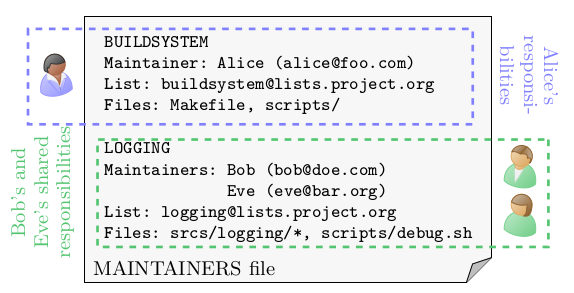
\includegraphics[scale=0.5]{Bilder/section-example}
	\end{frame}

	\begin{frame}
	\frametitle{MAINTAINERS-Datei}
	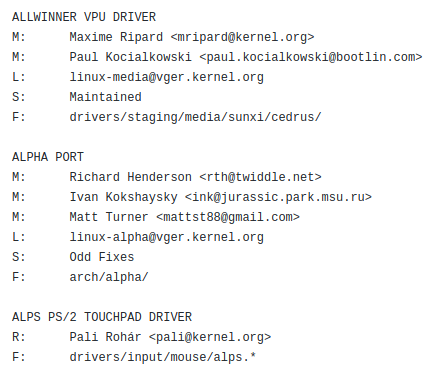
\includegraphics[scale=0.5]{Bilder/MAINTAINERSbild.png}
	\end{frame}

	%\begin{frame}
	%\frametitle{Das Subsystemproblem}
	%	\begin{block}{Was ist eigentlich ein Subsystem?}
	%		\begin{itemize}
	%			\item Bekannter Begriff, aber widersprüchliche Definitionen
	%			\item Die einzelnen Einträge in MAINTAINERS?
	%			\item Gruppierungen von MAINTAINERS Einträgen?
	%			\item Andere Einteilungen, die nirgendwo direkt stehen?
	%		\end{itemize}

	%	\end{block}
	%\end{frame}

	%\begin{frame}
	%\frametitle{Das Subsystemproblem}
	%	\begin{block}{Definition: Subsystem}
	%		Die Einträge in MAINTAINERS sind \textbf{Sektionen}.

	%		Zwei Sektionen sind \textbf{thematisch verwandt}, wenn sie viel Dateiinhalt teilen (LoC).

	%		Ein Subsystem ist eine \textbf{Gruppierung von thematisch stark verwandten Sektionen}.
	%	\end{block}

	%	\begin{alertblock}{Architektur-Distillierung}
	%		$\Rightarrow$ Architektur mithilfe von thematisch verwandten Sektionen distillieren
	%	\end{alertblock}
	%\end{frame}

	%\begin{frame}
	%\frametitle{Konforme Integration: alle Listen}
	%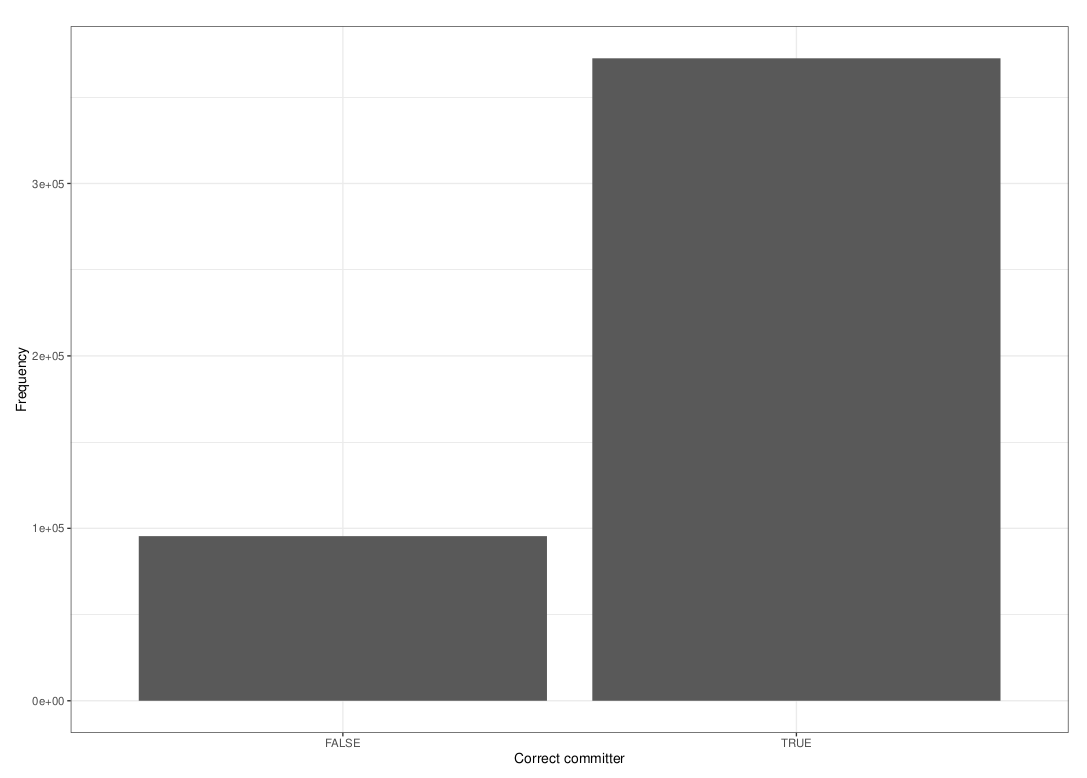
\includegraphics[scale=0.3]{Bilder/ResultatAlleListen.png}
	%\end{frame}

	\begin{frame}
	\frametitle{Methodik: Von Micro zu Macro}
	\centering
	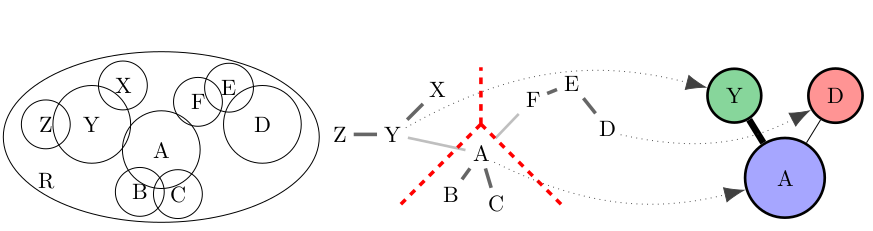
\includegraphics[scale=0.3]{Bilder/areasToMacro.png}
	\end{frame}

	\begin{frame}
	\frametitle{MAINTAINERS Verantwortlichkeitsbereiche}
	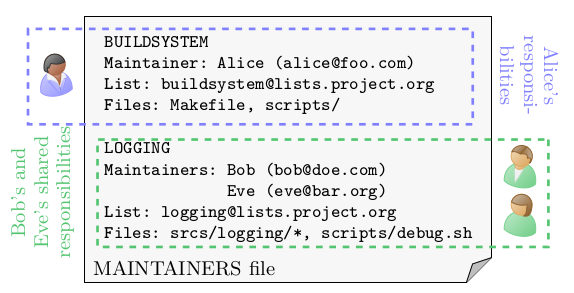
\includegraphics[scale=0.5]{Bilder/section-example}
	\end{frame}

	\begin{frame}
	\frametitle{Die Micro-View}
		\begin{block}{Architekturüberblick: Micro-View}
			\begin{itemize}
				\item Ungerichteter Graph, der Verantwortlichkeitsbereiche darstellt
				\item Jeder Knoten: ein Bereich
				\item Je größer der Bereich, desto größer der Knoten
				\item Zwei Bereiche teilen sich Verantwortlichkeiten $\Rightarrow$ Kante
				\item Je mehr geteilte Verantwortlichkeiten, je dicker die Kante
			\end{itemize}
		\end{block}
	\end{frame}

	\begin{frame}
	\frametitle{Micro-View: Xen-Project RELEASE-4.15.0}
	\centering
	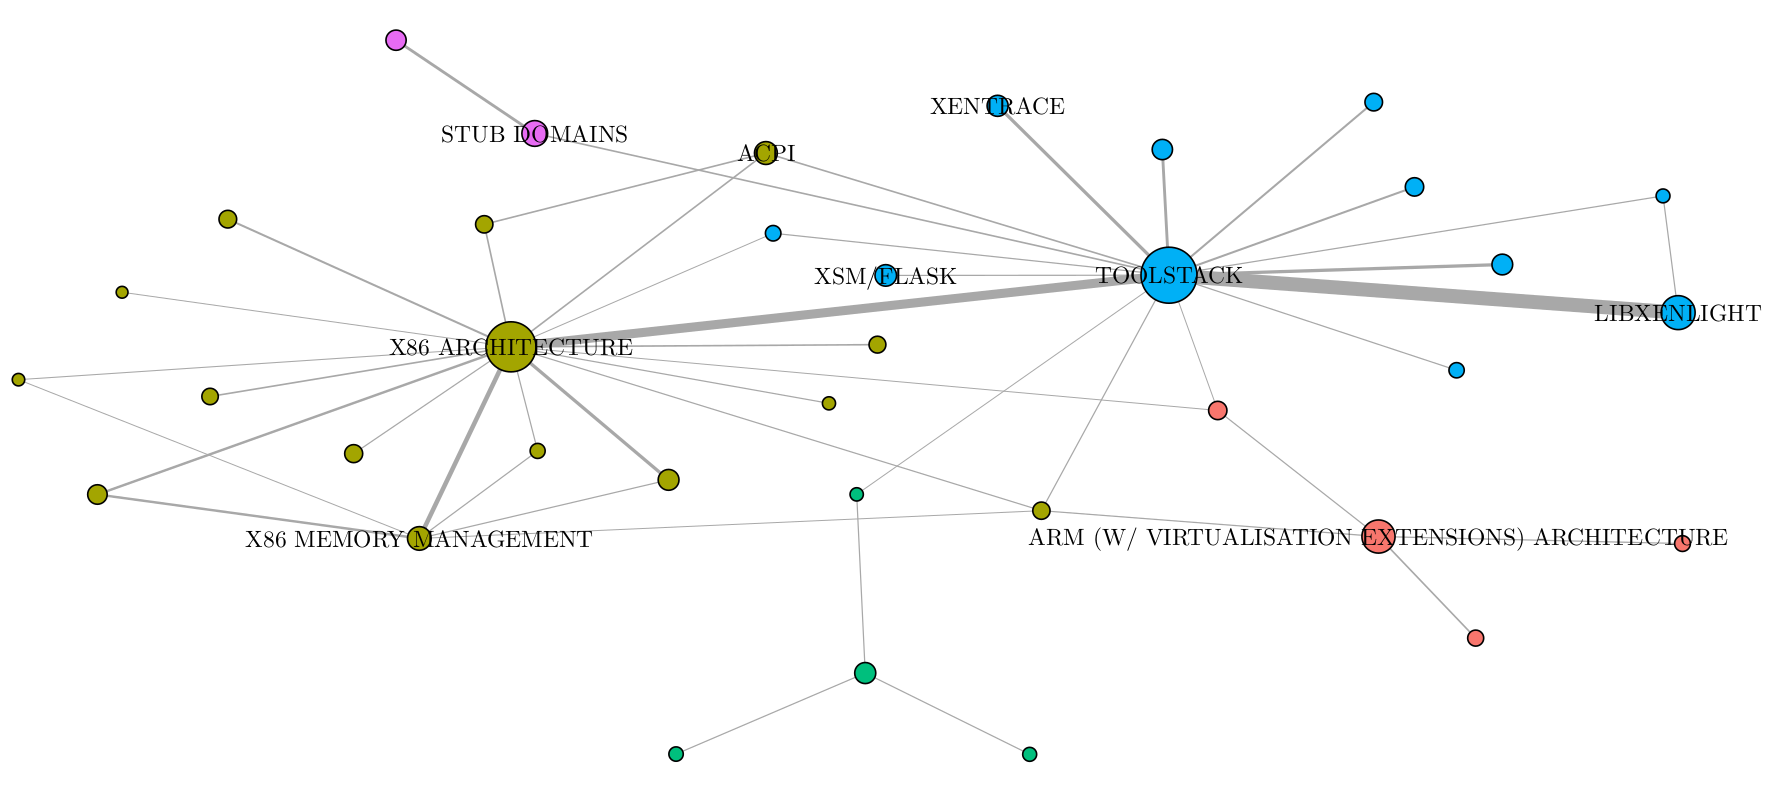
\includegraphics[scale=0.15]{Bilder/networkView}
	\end{frame}

	\begin{frame}
	\frametitle{Die Network-View}
		\begin{block}{Clusteruntersuchung: Network-View}
			\begin{itemize}
				\item Auf Cluster reduzierte Ansicht einer Micro-View
				\item Knoten außerhalb des Clusters nicht dargestellt
			\end{itemize}
		\end{block}
	\end{frame}


	\begin{frame}
	\frametitle{Network-View: Security für Linux}
	\centering
	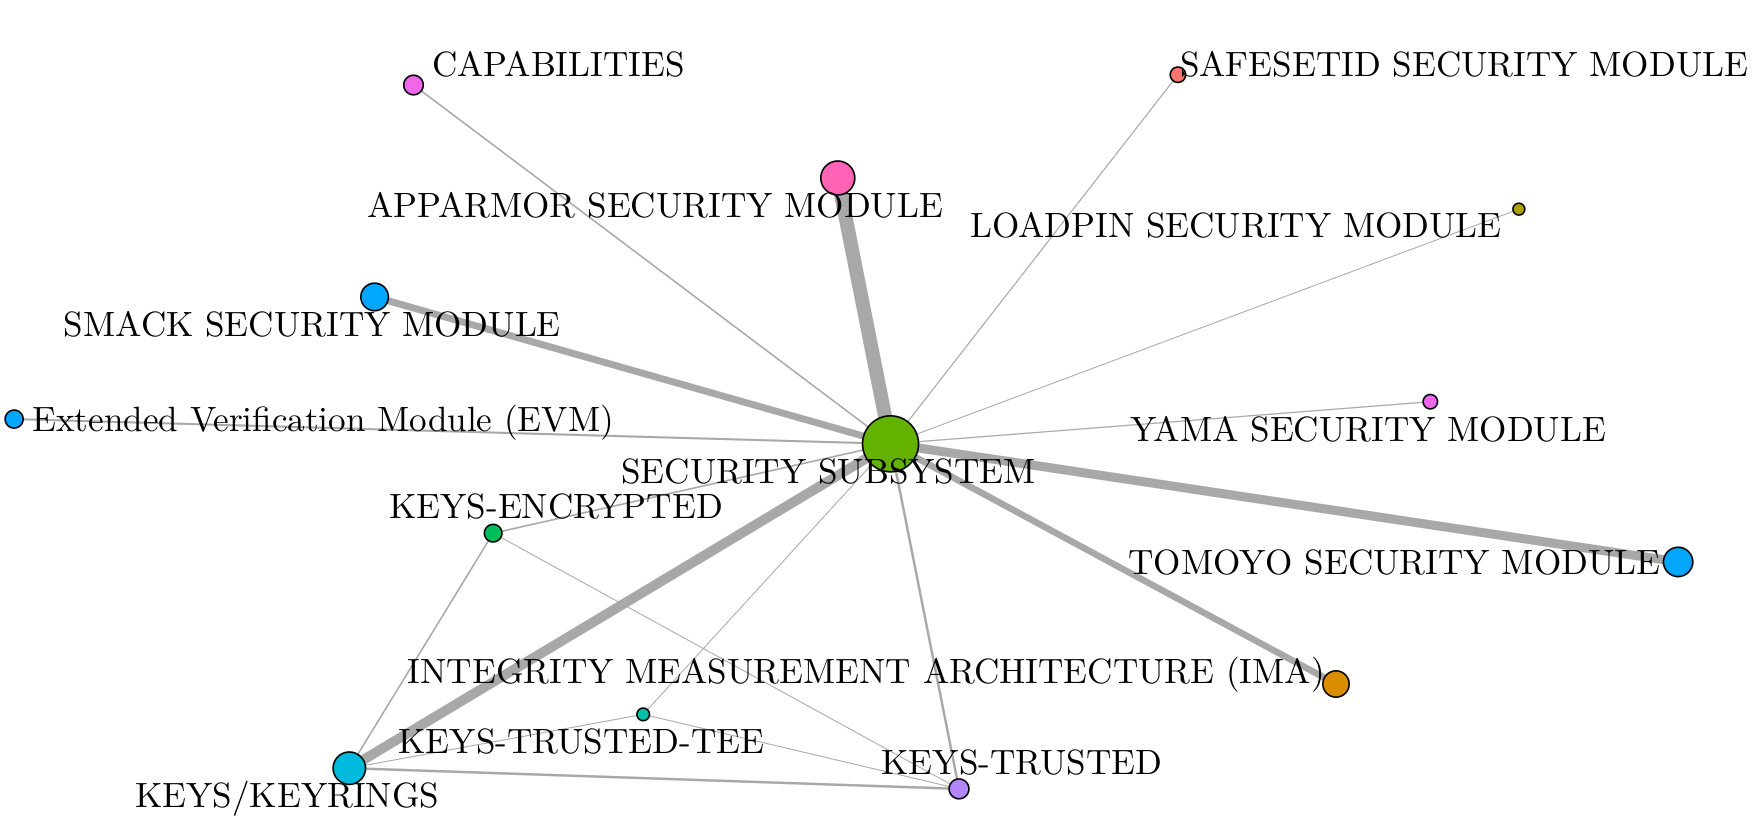
\includegraphics[scale=0.15]{Bilder/security}
	\end{frame}

	\begin{frame}
	\frametitle{Die Macro-View}
		\begin{block}{Übergeordnete Struktur: Macro-View}
			\begin{itemize}
				\item Jedes Cluster in Micro-View: ein Knoten
				\item Kanten zwischen Knoten: Kanten zwischen Clustern in Micro-View
			\end{itemize}
		\end{block}
	\end{frame}

	\begin{frame}
	\frametitle{Methodik: Von Micro zu Macro}
	\centering
	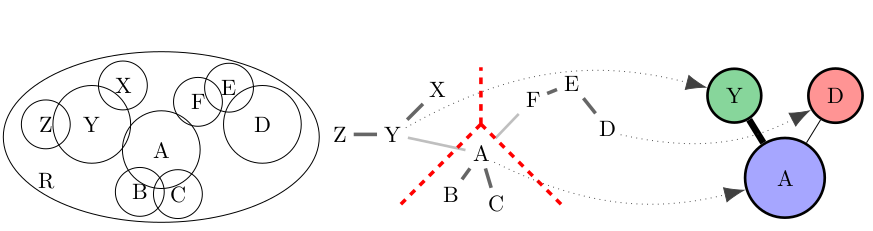
\includegraphics[scale=0.3]{Bilder/areasToMacro.png}
	\end{frame}


	\begin{frame}
	\frametitle{Macro-View: Linux über die Jahre}
	\centering
	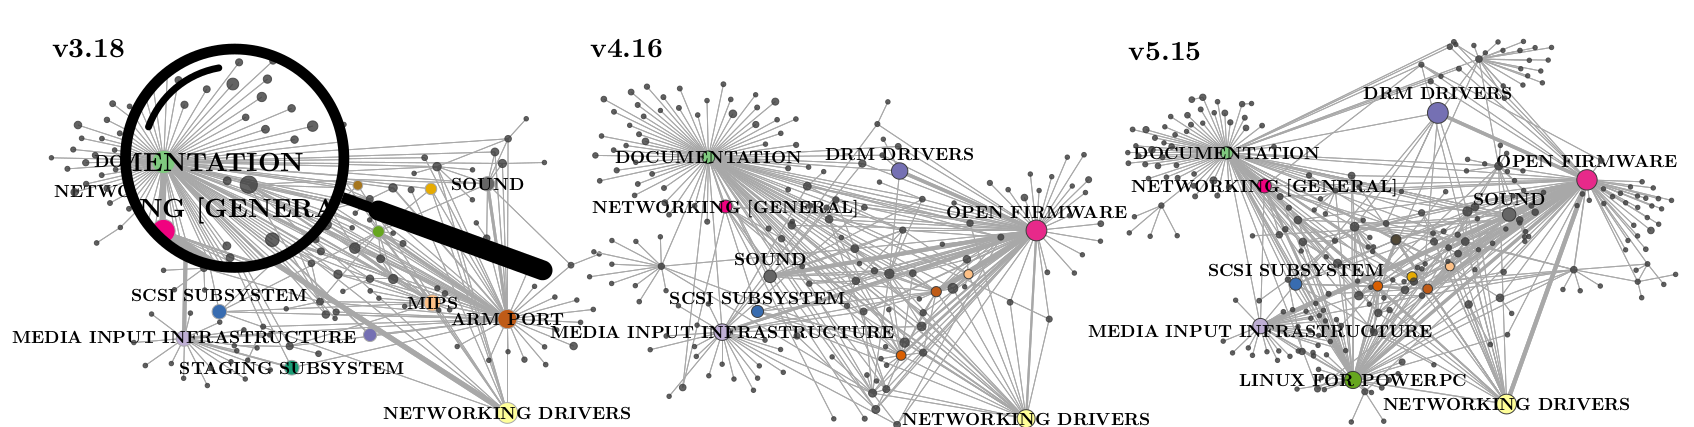
\includegraphics[scale=0.19]{Bilder/daumenkino}
	\end{frame}

	\begin{frame}
	\frametitle{Integrationsanalysen}
		\begin{center}
			\Huge Usecase für Methodik: Integrationsanalysen
		\end{center}
		%\begin{center}
		%	\begin{enumerate}
		%		\item get\_maintainer.pl Skript
		%		\item MAINTAINERS-Datei
		%	\end{enumerate}
		%\end{center}
		
	\end{frame}


	\begin{frame}
	\frametitle{Motivation}
	\begin{block}{Safety-Zertifikate}
		\begin{itemize}
			\item Sicherheitskritische Software kann Unterschied zwischen Leben und Tod sein
			\item Funktionalität muss sichergestellt werden
		\end{itemize}
	\end{block}
	\begin{block}{Sicherheit durch Prozess}
		\begin{itemize}
			\item Annahme: guter Entwicklungsprozess $\Rightarrow$ gute Software
			\item Entwickler müssen sich an Entwicklungsprozess halten
		\end{itemize}
	\end{block}
	\centering

	\end{frame}

	\begin{frame}
	\frametitle{OSS in Safety-Critical Environments}
	\begin{block}{Herausforderung: Zertifikate}
		\begin{itemize}
			\item OSS Software für seine Qualität bekannt
			\item Annahme: geeignet für sicherheitskritische Software
			\item Problem: Beweis für Entwicklungsprozesseinhaltung
		\end{itemize}
	\end{block}

	\centering
	Offene Entwicklungsprozesse sind gut definiert, aber wie gut halten sich die Entwickler daran?

	$\Rightarrow$ Entwicklungsprozess im Nachhinein analysieren
	\end{frame}

	\begin{frame}
	\frametitle{Mögliche Gründe für unkonforme Integration}
	\begin{block}{Zwei ,,falsche" Committer...}
		\begin{itemize}
			\item Daniel Vetter, Maintainer für \textit{DRM DRIVERS} und \textit{DRM DRIVER FOR VIRTUAL KERNEL MODESETTING (VKMS)}
			\item Maarten Lankhorst, Maintainer für \textit{DRM DRIVERS AND MISC GPU PATCHES}
		\end{itemize}
	\end{block}
	\begin{block}{... haben integriert für:}
		\begin{itemize}
			\item \textit{INTEL DRM DRIVERS (excluding Poulsbo, Moorestown and derivative chipsets)}
			\item \textit{INTEL GVT-g DRIVERS (Intel GPU Virtualization)} $\Rightarrow$ relevante Dateien in drivers/gpu/drm/i915/gvt/
		\end{itemize}
	\end{block}
	\end{frame}

	\begin{frame}
	\frametitle{Mögliche Gründe für unkonforme Integration}
	Florian Fainelli $\Rightarrow$ ,,Fälschlicherweise" committed für BROADCOM IPROC ARM ARCHITECTURE, wofür er \textbf{kein} Maintainer ist.
	\begin{block}{Florian Fainelli's Verantwortungsbereich}

		Florian Fainelli \textbf{ist} Maintainer für:
		\begin{itemize}
			\item BROADCOM B53 ETHERNET SWITCH DRIVER
			\item BROADCOM BCM63XX ARM ARCHITECTURE
			\item BROADCOM BCM7XXX ARM ARCHITECTURE
			\item BROADCOM BMIPS MIPS ARCHITECTURE
			\item ...
		\end{itemize}
	\end{block}

	$\Rightarrow$ Stichproben zeigen, dass sachverwandte Maintainers oft ,,falsch" committen, jedoch vermutlicherweise kein schlimmer/ungewollter Verstoß

	$\Rightarrow$ Relaxion notwendig für präzise Definition von Integrationen
	\end{frame}

	\begin{frame}
	\frametitle{Konformanzdefinitionen}
		\begin{block}{Ein Patch ist...}
			\begin{enumerate}
				\item \textbf{konform} integriert, wenn er von einem direkt zuständigen Maintainer integriert wurde
				\item \textbf{quasi-konform} integriert, wenn er von einem verwandten Maintainer integriert wurde
				%\item Listenrelevanz berücksichtigen
				\item \textbf{nicht-konform} integriert, wenn er von einem fachfremden Maintainer integriert wurde
			\end{enumerate}
		\end{block}
	\end{frame}

	\begin{frame}
	\frametitle{Methodik: Von Micro zu Macro}
	\centering
	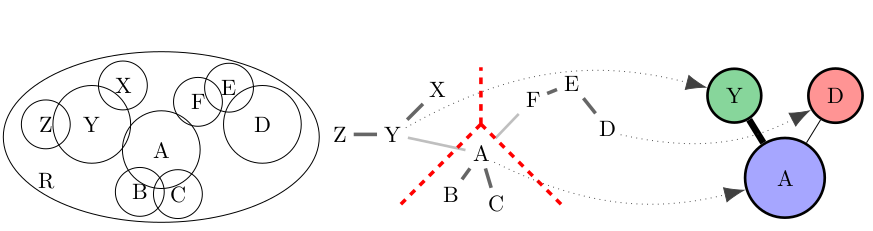
\includegraphics[scale=0.3]{Bilder/areasToMacro.png}
	\end{frame}


	\begin{frame}
	\frametitle{Konformanzdefinitionen}
		\begin{block}{Ein Patch ist...}
			\begin{enumerate}
				\item \textbf{micro-level konform} integriert, wenn er von einem direkt zuständigen Maintainer integriert wurde
				\item \textbf{macro-level konform} integriert, wenn er von einem verwandten Maintainer \textbf{in demselben Cluster} integriert wurde
				%\item Listenrelevanz berücksichtigen
				\item \textbf{nicht-konform} integriert, wenn er von einem fachfremden Maintainer integriert wurde
			\end{enumerate}
		\end{block}

	\end{frame}

	%kj\begin{frame}
	%kj\frametitle{Network-View: Security für Linux}
	%kj\centering
	%kj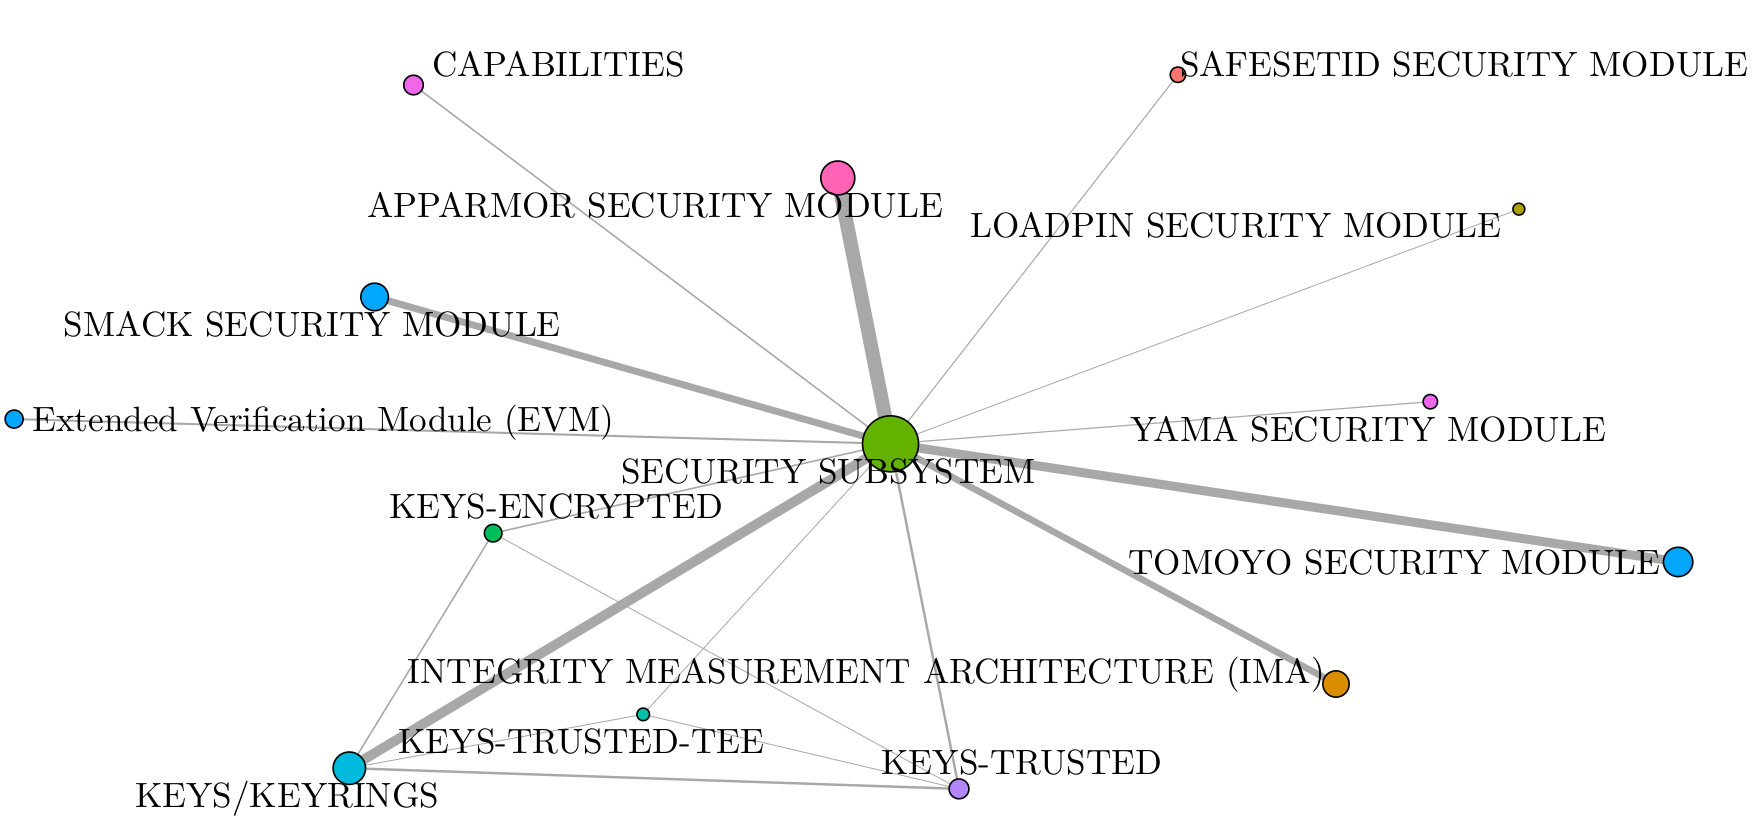
\includegraphics[scale=0.15]{Bilder/security}
	%kj\end{frame}


	\begin{frame}
	\frametitle{Konformanz über die Jahre: Projekte}
	\centering
	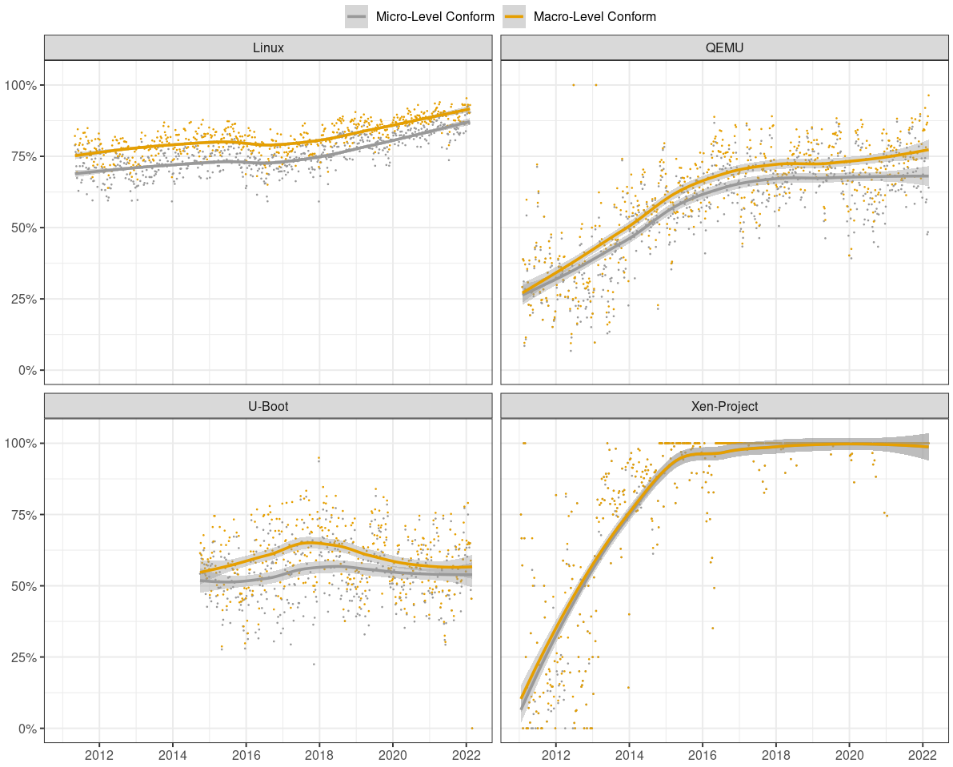
\includegraphics[scale=0.3]{Bilder/KonformanzAlle}
	\end{frame}

	\begin{frame}
	\frametitle{Konformanz über die Jahre: Linux auf Feature-Level}
	\centering
	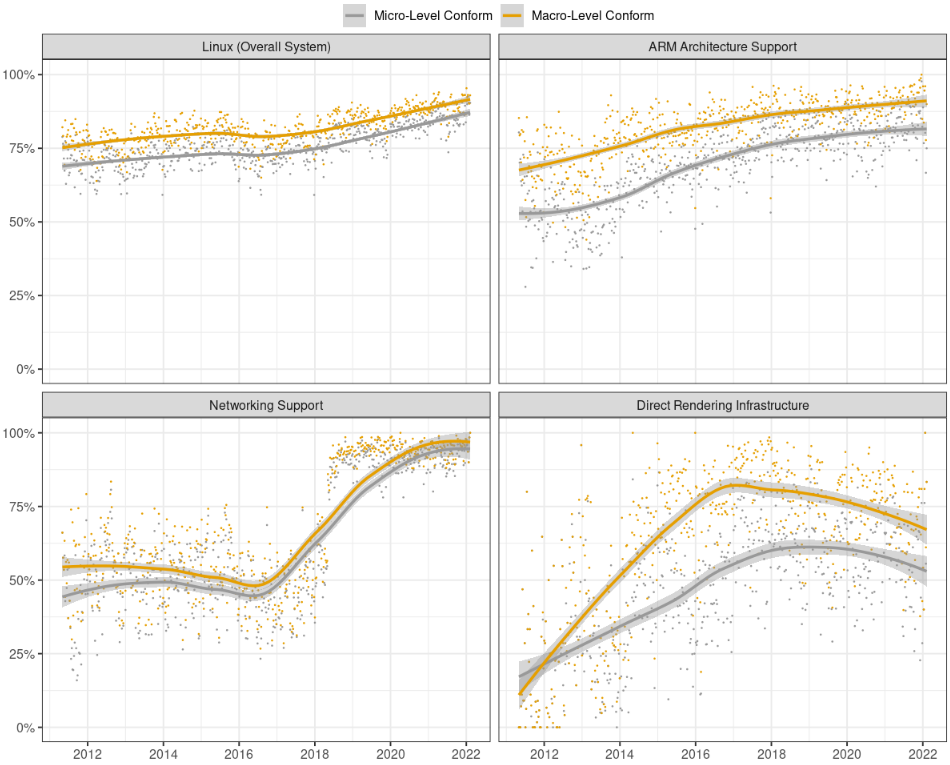
\includegraphics[scale=0.3]{Bilder/KonformanzLinux}
	\end{frame}
	%\begin{frame}
	%\frametitle{Möglich Gründe für unkonforme Integration}

	%\begin{block}{Listenrelevanz durch Adressierung}
	%	Patch auf Liste, später integriert $\Rightarrow$ von Analyse berücksichtigt
	%\end{block}

	%\begin{alertblock}{Unrelevante Liste?}
	%	Patch eigentlich unrelevant, aber dennoch gezählt

	%	Verfälschung der Daten?
	%\end{alertblock}
	%\end{frame}


	%\begin{frame}
	%\frametitle{Mögliche Gründe für unkonforme Integration}
	%	\begin{block}{Veraltete Maintainers}
	%		MAINTAINERS als \textbf{Ground Truth} definiert, aber nicht immer aktuell
	%		\\
	%		"[MAINTAINERS] tends to not always be up to date, though ..." 
	%	\end{block}
	%	%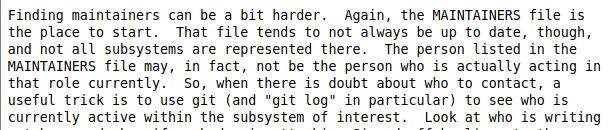
\includegraphics[scale=0.5]{Bilder/OutdatedMaintainers.png}
	%\end{frame}

	%\begin{frame}
	%\frametitle{Erweiterungen}
	%	\begin{block}{Raum für erweiternde Forschung}
	%		\begin{itemize}
	%			\item Entwicklung über Zweitverläufe hinweg
	%			\item Toleranz für Integration 
	%			%\item Listenrelevanz berücksichtigen
	%			\item ...
	%		\end{itemize}
	%	\end{block}
	%\end{frame}

	\begin{frame}
	\frametitle{Ende}
	\Huge
	\centering
	Danke fürs Zuhören!
	\end{frame}
	%\begin{frame}
	%\frametitle{Konformanz über die Jahre: Linux auf Feature-Level}
	%\centering
	%\includegraphics[scale=0.2]{Bilder/linuxOverall}
	%\end{frame}
\end{document}
